%%% Template originaly created by Karol Kozioł (mail@karol-koziol.net) and modified for academic use by Shahidh K Muhammed (shahidhkmuhammed@gmail.com)

\documentclass[a4paper,11pt]{article}

\usepackage[T1]{fontenc}
\usepackage[utf8]{inputenc}
\usepackage{graphicx}
\graphicspath{ {img/} }
\usepackage{xcolor}

%\renewcommand\familydefault{\sfdefault}

\usepackage{tgheros}
\usepackage[defaultmono]{droidmono}

\usepackage{amsmath,amssymb,amsthm,textcomp}
\usepackage{enumerate}
\usepackage{multicol}
\usepackage{tikz}

\usepackage{geometry}
\geometry{total={210mm,297mm},
left=25mm,right=25mm,%
bindingoffset=0mm, top=20mm,bottom=20mm}


\linespread{1.3}

\newcommand{\linia}{\rule{\linewidth}{0.5pt}}


% custom theorems if needed
\newtheoremstyle{mytheor}
    {1ex}{1ex}{\normalfont}{0pt}{\scshape}{.}{1ex}
    {{\thmname{#1 }}{\thmnumber{#2}}{\thmnote{ (#3)}}}

\theoremstyle{mytheor}
\newtheorem{defi}{Definition}

% my own titles
\makeatletter
\renewcommand{\maketitle}{
\begin{center}
\vspace{2ex}
{\huge \textsc{\@title}}
\vspace{1ex}
\\
\linia\\
\@author \hfill \@date
\vspace{4ex}
\end{center}
}
\makeatother
%%%

% custom footers and headers
\usepackage{fancyhdr}
\pagestyle{fancy}
\lhead{}
\chead{}
\rhead{}
\lfoot{Assignment \textnumero{} 1}
\cfoot{}
\rfoot{Page \thepage}
\renewcommand{\headrulewidth}{0pt}
\renewcommand{\footrulewidth}{0pt}
%

% code listing settings
\usepackage{listings}
\lstset{
    language=Java,
    basicstyle=\ttfamily\small,
    aboveskip={1.0\baselineskip},
    belowskip={1.0\baselineskip},
    columns=fixed,
    extendedchars=true,
    breaklines=true,
    tabsize=4,
    prebreak=\raisebox{0ex}[0ex][0ex]{\ensuremath{\hookleftarrow}},
    frame=lines,
    showtabs=false,
    showspaces=false,
    showstringspaces=false,
    keywordstyle=\color[rgb]{0.627,0.126,0.941},
    commentstyle=\color[rgb]{0.133,0.545,0.133},
    stringstyle=\color[rgb]{01,0,0},
    numbers=left,
    numberstyle=\small,
    stepnumber=1,
    numbersep=10pt,
    captionpos=t,
    escapeinside={\%*}{*)}
}

%%%----------%%%----------%%%----------%%%----------%%%

\begin{document}

\title{Programming Assignment \textnumero{} 1}

\author{RollNo - Name}

\date{Jan 2017}

\maketitle


\section{}

A question can be answered here.
\subsection{}

This is how a sub-question can be answered.

Write explanations here. You can refer to code like this: Listing~\ref{code:stackinterface}. Add inline code with monospace font like this: \texttt{ArrayStack}.



\begin{lstlisting}[label={code:stackinterface},caption=Stack interface in Java]
public interface Stack<E> {
    /**
    * Return the number of elements in the stack.
    * @return number of elements in the stack.
    */
    public int size();
    /**
    * Return whether the stack is empty.
    * @return true if the stack is empty, false otherwise.
    */
    public boolean isEmpty();
    /**
    * Inspect the element at the top of the stack.
    * @return top element in the stack.
    * @exception EmptyStackException if the stack is empty.
    */
    public E top()
        throws EmptyStackException;
    /**
    * Insert an element at the top of the stack.
    * @param element to be inserted.
    */
    public void push (E element);
    /**
    * Remove the top element from the stack.
    * @return element removed.
    * @exception EmptyStackException if the stack is empty.
    */
    public E pop()
        throws EmptyStackException;
}
\end{lstlisting}


\subsection{Another Sub Question}

More explanations

\section{}

Another question can be answered here.

This is how an image can be added:

Upload the image to img folder and refer to it as Figure \ref{fig:sampletree}
\begin{figure}[h]
\caption{Sample tree}
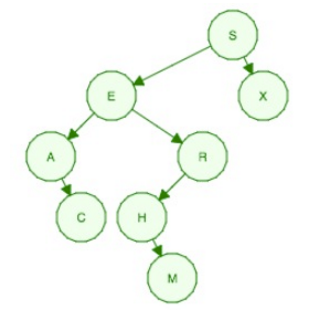
\includegraphics[scale=.6]{sampletree}
\centering
\label{fig:sampletree}
\end{figure}

\end{document}
